\chapter{Асимптотика собственных значений}\label{ch:ch2}
\section{Квантовый биллиард в эллиптическом кольце и
накрытии эллиптического кольца}\label{sec:ch2/sec1}
Введем функцию 
\begin{equation}
W_{a, b}(u) = Y_a(u)J_b(\lambda u) - Y_a(\lambda u)J_b(u), \quad \lambda = \frac{r_1}{r_0}. 
%\tag{5}
\label{eq:YJdef}
\end{equation}

Обозначим $\nu = \frac{k}{p}, k \in \mathbb{Z}$. 
\begin{theorem}
	Значение $\varkappa^2_{k,m}(\delta), k, m \in \mathbb{N}$, зависит от половины фокусного расстояния $\delta$ с точностью до $o(\delta^2)$ следующим образом:
{\small
\begin{equation}
\varkappa^2_{k,m}(\delta) = \left[
\begin{array}{cc}
\dfrac{\alpha_{\nu, m}^2}{r_0^2} + \delta^2 \dfrac{\alpha_{\nu, m}^3}{8 \nu r_0^4} \left. \frac{
\frac{\nu-2}{\nu-1}
\left(
W_{\nu-2, \nu}(u) + W_{\nu, \nu-2}(u)
\right)- 
\frac{\nu+2}{\nu+1}
\left(
W_{\nu+2, \nu}(u) + W_{\nu, \nu+2}(u)
\right)
}{ \frac{\partial W_{\nu,\nu}(u)}{\partial u} }\right|_{u=\alpha_{\nu, m}},  & -\nu \in \mathbb{N} \setminus \{1, 2\}; \\

\dfrac{\alpha_{2, m}^2}{r_0^2} - \delta^2 \dfrac{\alpha_{2, m}^3}{12  r_0^4} \left. \frac{
	\left(
	W_{4, 2}(u) + W_{2, 4}(u)
	\right)
}{ \frac{\partial W_{2,2}(u)}{\partial u} }\right|_{u=\alpha_{2, m}}, & -\nu=2; \\

\dfrac{\alpha_{1, m}^2}{r_0^2} - \delta^2 \dfrac{3 \alpha_{1, m}^3 }{16 r_0^4}
\left. \frac{
	\left(
	W_{3, 1}(u) + W_{1, 3}(u)
	\right)
}{ \frac{\partial W_{1,1}(u)}{\partial u} }\right|_{u=\alpha_{1, m}}, & -\nu=1; \\


\dfrac{\alpha_{0, m}^2}{r_0^2} - \delta^2 \dfrac{\alpha_{0, m}^3}{4r_0^4} \left. \frac{
 \left( W_{2, 0}(u) + W_{0, 2}(u) \right)
}{ \frac{\partial W_{0,0}(u)}{\partial u} }\right|_{u=\alpha_{0, m}}, & \nu=0;   \\

\dfrac{\alpha_{1, m}^2}{r_0^2} - \delta^2 \dfrac{\alpha_{1, m}^3}{16 r_0^4} \left. \frac{ \left( W_{3, 1}(u) + W_{1, 3}(u) \right)
}{ \frac{\partial W_{1,1}(u)}{\partial u} }\right|_{u=\alpha_{1, m}},    & \nu=1;\\

\dfrac{\alpha_{\nu, m}^2}{r_0^2} + \delta^2 \dfrac{\alpha_{\nu, m}^3}{2 r_0^4} \left. \frac{
\frac{1}{4(\nu-1)} \left( W_{\nu-2, \nu}(u) + W_{\nu, \nu-2}(u) \right) - \frac{1}{4(\nu+1)} \left( W_{\nu+2, \nu}(u) + W_{\nu, \nu+2}(u) \right)
}{ \frac{\partial W_{\nu,\nu}(u)}{\partial u} }\right|_{u=\alpha_{\nu, m}},
&   \left[
\begin{aligned}
\nu &\in \mathbb{N} \setminus \{1\},\\
\nu &\notin \mathbb{Z}.
\end{aligned}
\right.
\end{array}
\right.,
%\tag{6}
\label{eq:valRing}
\end{equation}
}
где $\alpha_{\nu, m}$ --- $m$-й нуль функции $W_{\nu, \nu}(u)$.
\label{th:sect2_th4}
\end{theorem}


\begin{remark}
Это разложение равносильно разложению по эксцентриситету $\varepsilon_s$ внутреннего или внешнего эллипса с большой полуосью $r_s, s = 0, 1$, которое получается из подстановки $\delta = \varepsilon_s r_s$.
\end{remark}

\begin{remark}
Случай $\delta=0$ соответствует накрытию кругового кольца. Легко видеть, что в этом случае результат теоремы \ref{th:sect2_th4}  (т.е. нулевые члены разложений) после умножения на $\frac{\hbar^2}{2M}$ соответствует результату теоремы \ref{th:sect1_theorem1}.
\end{remark}

\begin{remark}
Производная $\frac{\partial W_{\nu, \nu}(u)}{\partial u}$ допускает выражение через функции Бесселя первого и второго рода.
Имеем тождества (см. \cite{wref5}): 
$2\frac{\partial Y_\nu(u)}{\partial u} = Y_{\nu-1}(u) - Y_{\nu+1}(u)$, $2\frac{\partial J_\nu(u)}{\partial u} = J_{\nu-1}(u) - J_{\nu+1}(u)$.
Непосредственным дифференцированием 
$W_{\nu, \nu}(u)$ получаем
$$\frac{\partial W_{\nu, \nu}(u)
}{\partial u} = 
\lambda \big(Y_\nu(u) J_{\nu-1}(\lambda u)
+  Y_{\nu+1}(\lambda u) J_\nu(u)\big) - 
\big(Y_\nu(\lambda u) J_{\nu-1}(u)  + 
 Y_{\nu+1}(u) J_\nu(\lambda u) \big).$$
 \end{remark}

По предыдущей теореме \ref{th:sect2_th3} собственные значения $E_{k, m}$ оператора $\hat{H}$, а следовательно, числа $\varkappa^2_{k,m} = \varkappa^2_{k,m}(\delta)$ связаны с нулями $\beta_{\nu, m}$ функции $f(q)$. Здесь функция $f(q)$ имеет один из трех возможных видов (см. \eqref{eq:funcF}).

Приведем две леммы, с помощью которых докажем теорему \ref{th:sect2_th4}.
\medskip

Пусть $\nu = \frac{k}{p}, k \geq 0, \zeta = \lambda_\nu(q), q=\frac{\varkappa^2 \delta^2}{4}$, и пусть $ce_\nu(\phi, q)$ --- четное решение углового уравнения Матьё с указанными параметрами $\zeta, q$. Напомним, что для малых $q$ справедливо разложение (см. \cite[\S~2.2, с.~122---124]{wref12}):
$$ce_\nu(\phi, q) = c_\nu \cos{\nu \phi} + q c_{\nu+2} \cos{(\nu+2) \phi} +q c_{\nu-2} \cos{(\nu-2) \phi} + o(q).$$ 

Возможные значения $\varkappa^2$ определяются из условия обращения в нуль радиальной функции Матьё на граничных эллипсах. А именно положим 
$R(\rho)$ решением радиального уравнения Матьё с этими же параметрами и граничным условием $R(\rho_0)=R(\rho_1)=0$, $\rho_0 < \rho_1$. 
\begin{lemma}
Пусть $r_0 = \delta\cosh{\rho_0}, r_1 = \delta\cosh{\rho_1}, \lambda = \frac{r_1}{r_0}$, $\alpha_{\nu, m}$ --- $m$-й нуль функции $W_{\nu, \nu}(u)$. Тогда $\varkappa^2$ при малых $\delta$ имеет вид
\begin{multline*}
\varkappa^2 = \dfrac{\alpha_{\nu, m}^2}{r_0^2} + \delta^2 \dfrac{\alpha_{\nu, m}^3}{2 c_\nu r_0^4} \times \\ \times \left. \frac{
c_{\nu+2} \left( W_{\nu+2, \nu}(u) + W_{\nu, \nu+2}(u) \right) + 
c_{\nu-2} \left( W_{\nu-2, \nu}(u) + W_{\nu, \nu-2}(u) \right)
}{ \frac{\partial W_{\nu,\nu}(u)}{\partial u} }\right|_{u=\alpha_{\nu, m}} + o(\delta^2).
\end{multline*}
\label{th:ringLemma1}
\end{lemma}

\begin{proof}
При $\zeta = \lambda_\nu(q), \nu = \frac{k}{p}, k \geq 0$ коэффициенты разложения Фурье четной угловой функции Матьё $ce_\nu(\phi, q)$ связаны \cite{wref2} с точностью до постоянного множителя с разложением радиальной функции Матьё $R_1(\rho, q) = \left[
\begin{array}{ll}
    Ce_\nu(\rho, q),     & \nu \in \{0\} \cup \mathbb{N};  \\
    M_\nu^{(1)}(\rho, q), & \nu \notin \mathbb{Z},
\end{array}
\right.$ в бесконечную сумму функций Бесселя следующим образом:
$$ R_1(\rho, q) = 
	c_\nu J_\nu(2\sqrt{q}\cosh{\rho}) - 
	q c_{\nu-2} J_{\nu-2}(2\sqrt{q}\cosh{\rho}) -
	q c_{\nu+2} J_{\nu+2}(2\sqrt{q}\cosh{\rho}) + o(q).$$

Второе решение $R_2(\rho, q)$  радиального уравнения Матьё можно получить из $R_1(\rho, q)$ заменой функций Бесселя первого рода $J_\nu(x)$ на функции Бесселя второго рода $Y_\nu(x)$. В частности, это будут функции $Fey_\nu(\rho, q)$ при $\nu \in \{0\} \cup \mathbb{N}$ и $M_\nu^{(2)}(\rho, q)$ при $\nu \in \mathbb{Q} \setminus \mathbb{Z}, \nu \ge 0$.

Напомним граничное условие $R_2(\rho_0) R_1(\rho_1) - R_2(\rho_1) R_1(\rho_0) = 0$. Заметим, что аргументы имеют вид $2 \sqrt{q} \cosh{\rho_s} = 2 \sqrt{\frac{\varkappa^2 \delta^2}{4}} \frac{r_s}{\delta} = \varkappa r_s, s=0,1$. Рассмотрим первое слагаемое в граничном условии:
\begin{multline}
	R_2(\rho_0) R_1(\rho_1) = \\
\bigg(
c_\nu Y_\nu(\varkappa r_0) - 
	q c_{\nu-2} Y_{\nu-2}(\varkappa r_0) -
	q c_{\nu+2} Y_{\nu+2}(\varkappa r_0) + o(q)
\bigg) \times \\
\times \bigg(
c_\nu J_\nu(\varkappa r_1) - 
	q c_{\nu-2} J_{\nu-2}(\varkappa r_1) -
	q c_{\nu+2} J_{\nu+2}(\varkappa r_1) + o(q)
\bigg) = \\
= c_\nu^2 Y_\nu(\varkappa r_0)J_\nu(\varkappa r_1) - 
	q c_\nu \bigg(    c_{\nu-2} 
	\big(
	Y_{\nu-2}(\varkappa r_0)J_\nu(\varkappa r_1) + Y_{\nu}(\varkappa r_0)J_{\nu-2}(\varkappa r_1)
	\big)+ \\
	  +  c_{\nu+2} 
	\big(
	Y_{\nu+2}(\varkappa r_0)J_\nu(\varkappa r_1) + Y_{\nu}(\varkappa r_0)J_{\nu+2}(\varkappa r_1)
	\big)
\bigg) + o(q).
%\tag{7}
\label{eq:eqRR}
\end{multline}
Разделив обе части последнего выражения на $c_\nu^2$, для удобства определим $u = \varkappa r_0, \lambda = \frac{r_1}{r_0}, \varkappa r_1 = \lambda u$. Запишем полное выражение $R_2(\rho_0) R_1(\rho_1) - R_2(\rho_1) R_1(\rho_0) = 0$: поскольку слагаемые отличаются друг от друга только перестановкой аргументов $u$ и $\lambda u$, использование формулы \eqref{eq:eqRR} приведет к появлению функций \eqref{eq:YJdef}. Таким образом,
\begin{multline}
	0 = R_2(\rho_0) R_1(\rho_1) - R_2(\rho_1) R_1(\rho_0)  =  W_{\nu, \nu}(u) - \\
	- q \bigg(    
	\frac{c_{\nu-2}}{c_\nu}
	\left(
	W_{\nu-2, \nu}(u) + W_{\nu, \nu-2}(u)
	\right)+ 
	\frac{c_{\nu+2}}{c_\nu}
	\left(
	W_{\nu+2, \nu}(u) + W_{\nu, \nu+2}(u)
	\right)
\bigg) + o(q).
%\tag{8}
\label{eq:25}
\end{multline}
Пусть $\alpha_{\nu, m}$ --- $m$-й нуль функции $W_{\nu, \nu}(u)$. Тогда в достаточно малой его окрестности справедливо 
$$
W_{\nu, \nu}(u) = (u - \alpha_{\nu, m}) \left.
\frac{\partial W_{\nu, \nu}(u)}{\partial u}
\right|_{u=\alpha_{\nu, m}} + 
\frac{ (u - \alpha_{\nu, m})^2 }{2} \left.
\frac{\partial^2 W_{\nu, \nu}(u)}{\partial u^2}
\right|_{u=\alpha_{\nu, m}} + o((u - \alpha_{\nu, m})^2).
$$

Положим $u = \alpha_{\nu, m} + u_1 \delta + u_2 \delta^2 + o(\delta^2)$ и подставим $q = \frac{\varkappa^2 \delta^2}{4} = \frac{u^2 \delta^2}{4 r_0^2}$ в выражение \eqref{eq:25}:
\begin{multline*}
    (u_1 \delta + u_2 \delta^2 + o(\delta^2)) 
\left.
\frac{\partial W_{\nu, \nu}(u)}{\partial u}
\right|_{u=\alpha_{\nu, m}} + 
    \frac{u_1^2 \delta^2 + o(\delta^2)}{2}
\left.
\frac{\partial^2 W_{\nu, \nu}(u)}{\partial u^2}
\right|_{u=\alpha_{\nu, m}} 
- \\ - \frac{\alpha_{\nu, m}^2 \delta^2 + o(\delta^2)}{4r_0^2}  \bigg[\bigg(    
	\frac{c_{\nu-2}}{c_\nu}
    \left(W_{\nu-2, \nu}(u) + W_{\nu, \nu-2}(u) \right)+ 
\\
+	\frac{c_{\nu+2}}{c_\nu}
	\left(
	W_{\nu+2, \nu}(u) + W_{\nu, \nu+2}(u)
	\right)
\left.
\bigg)
\right|_{u=\alpha_{\nu, m}}
+ o(\delta)
\bigg]
 + o(\delta^2) = 0.
 \end{multline*}
Поскольку равенство должно выполняться при каждой степени $\delta$, получаем в первую очередь $u_1 = 0$, затем, приравняв коэффициенты при $\delta^2$, заключаем, что
$$u_2 = \frac{\alpha_{\nu, m}^2}{4r_0^2} 
\left.
\frac{
	\frac{c_{\nu-2}}{c_\nu}
	\left(
	W_{\nu-2, \nu}(u) + W_{\nu, \nu-2}(u)
	\right)+
	\frac{c_{\nu+2}}{c_\nu}
	\left(
	W_{\nu+2, \nu}(u) + W_{\nu, \nu+2}(u)
	\right)
}{ \frac{\partial W_{\nu,\nu}(u)}{\partial u} }
\right|_{u=\alpha_{\nu, m}}.$$
Таким образом, 
{\small
\[
u = \alpha_{\nu, m} + \delta^2 \frac{\alpha_{\nu, m}^2}{4r_0^2} \left.
\frac{
	\frac{c_{\nu-2}}{c_\nu}
	\left(
	W_{\nu-2, \nu}(u) + W_{\nu, \nu-2}(u)
	\right)+
	\frac{c_{\nu+2}}{c_\nu}
	\left(
	W_{\nu+2, \nu}(u) + W_{\nu, \nu+2}(u)
	\right)
}{ \frac{\partial W_{\nu,\nu}(u)}{\partial u} }
\right|_{u=\alpha_{\nu, m}} + o(\delta^2). 
\]
}
Поскольку $u = \varkappa r_0$, получаем
{\small
\[
\varkappa^2 = \dfrac{\alpha_{\nu, m}^2}{r_0^2} + \delta^2 \dfrac{\alpha_{\nu, m}^3}{2 c_\nu r_0^4} \left. \frac{
c_{\nu+2} \left( W_{\nu+2, \nu}(u) + W_{\nu, \nu+2}(u) \right) + 
c_{\nu-2} \left( W_{\nu-2, \nu}(u) + W_{\nu, \nu-2}(u) \right)
}{ \frac{\partial W_{\nu,\nu}(u)}{\partial u} }\right|_{u=\alpha_{\nu, m}} + o(\delta^2).
\]
}

Лемма доказана.
\end{proof}
\medskip

Пусть $\zeta = \lambda_{-\nu}(q), \nu \in \mathbb{N}, q=\frac{\varkappa^2 \delta^2}{4}$, и пусть $se_\nu(\phi, q)$ --- нечетное решение углового уравнения Матьё с указанными параметрами $\zeta, q$.
Напомним, что для малых $q$ справедливо разложение (см. \cite[\S\ 2.2, с.~122--124]{wref12}):
$$se_\nu(\phi, q) = c_\nu \sin{\nu \phi} + q c_{\nu+2} \sin{(\nu+2) \phi} +q c_{\nu-2} \sin{(\nu-2) \phi} + o(q).$$ 
Возможные значения $\varkappa^2$ определяются из условия обращения в нуль радиальной функции Матьё на граничных эллипсах. А именно положим $R(\rho)$ решением радиального уравнения Матьё с этими же параметрами и граничным условием $R(\rho_0)=R(\rho_1)=0$, $\rho_0 < \rho_1$.
\begin{lemma}
Пусть $r_0 = \delta\cosh{\rho_0}, r_1 = \delta\cosh{\rho_1}, \lambda = \frac{r_1}{r_0}$, $\alpha_{\nu, m}$ --- $m$-й нуль функции $W_{\nu, \nu}(u)$, тогда $\varkappa^2$ зависит от $\delta$ как
{\small
\begin{multline*}
\varkappa^2 = \dfrac{\alpha_{\nu, m}^2}{r_0^2} + \delta^2 \dfrac{\alpha_{\nu, m}^3}{2 \nu c_\nu r_0^4} \times \\ \times \left. \frac{
	(\nu-2) c_{\nu-2}
	\left(
	W_{\nu-2, \nu}(u) + W_{\nu, \nu-2}(u)
	\right)+ 
    (\nu+2) c_{\nu+2}
	\left(
	W_{\nu+2, \nu}(u) + W_{\nu, \nu+2}(u)
	\right)
}{ \frac{\partial W_{\nu,\nu}(u)}{\partial u} }\right|_{u=\alpha_{\nu, m}} + o(\delta^2).
\end{multline*}
}
\label{th:ringLemma2}
\end{lemma}

\begin{proof}
При $\zeta = \lambda_{-\nu}(q), \nu \in \mathbb{N}$, коэффициенты разложения Фурье нечетной угловой функции Матьё $se_\nu(\phi, q)$ связаны \cite{wref2} с точностью до постоянного множителя с разложением радиальной функции Матьё $Se_\nu(\rho, q)$ в бесконечную сумму функций Бесселя следующим образом:
{\small
\[
Se_\nu(\rho, q) = 
	\nu c_\nu J_\nu(2\sqrt{q}\cosh{\rho})  -
	q (\nu-2) c_{\nu-2} J_{\nu-2}(2\sqrt{q}\cosh{\rho}) - 
	q (\nu+2) c_{\nu+2} J_{\nu+2}(2\sqrt{q}\cosh{\rho}) + o(q).
\]
}
Второе решение радиального уравнения Матьё $R_2(\rho)=Gey_\nu(\rho, q)$ можно получить из решения $R_1(\rho)=Se_\nu(\rho, q)$ заменой функций Бесселя первого рода $J_\nu(x)$ на функции Бесселя второго рода $Y_\nu(x)$.

В граничном условии $R_2(\rho_0) R_1(\rho_1) - R_2(\rho_1) R_1(\rho_0) = 0$ аргументы имеют вид $2 \sqrt{q} \cosh{\rho_s} = 2 \sqrt{\frac{\varkappa^2 \delta^2}{4}} \frac{r_s}{\delta} = \varkappa r_s, s=0,1$. Рассмотрим первое слагаемое:
{\small
\begin{multline*}
	R_2(\rho_0) R_1(\rho_1) = \\
=\big(
\nu c_\nu Y_\nu(\varkappa r_0) - 
	q (\nu-2) c_{\nu-2} Y_{\nu-2}(\varkappa r_0) -
	q (\nu+2) c_{\nu+2} Y_{\nu+2}(\varkappa r_0) + o(q)
\big) \times \\
\times \big(
\nu c_\nu J_\nu(\varkappa r_1) - 
	q (\nu-2) c_{\nu-2} J_{\nu-2}(\varkappa r_1) -
	q (\nu+2) c_{\nu+2} J_{\nu+2}(\varkappa r_1) + o(q)
\big) = \\
= \nu^2 c_\nu^2 Y_\nu(\varkappa r_0)J_\nu(\varkappa r_1) - 
	q \nu c_\nu \bigg(   (\nu-2) c_{\nu-2} 
	\big(
	Y_{\nu-2}(\varkappa r_0)J_\nu(\varkappa r_1) +  Y_{\nu}(\varkappa r_0)J_{\nu-2}(\varkappa r_1)
	\big) +
	\\ +
	 (\nu+2) c_{\nu+2} 
	\big(
	Y_{\nu+2}(\varkappa r_0)J_\nu(\varkappa r_1) + Y_{\nu}(\varkappa r_0)J_{\nu+2}(\varkappa r_1)
	\big)
\bigg) + o(q).
\end{multline*}
}
Разделим обе части выражения на $\nu^2 c_\nu^2$ и для удобства определим $u = \varkappa r_0, \lambda = \frac{r_1}{r_0}  \varkappa r_1 = \lambda u$. Запишем полное выражение $R_2(\rho_0) R_1(\rho_1) - R_2(\rho_1) R_1(\rho_0) = 0$ тем же способом, что и в лемме \ref{th:ringLemma1}:
\begin{multline}
	0 = R_2(\rho_0) R_1(\rho_1) - R_2(\rho_1) R_1(\rho_0)  = \\
= W_{\nu, \nu}(u) - 
	\frac{q}{\nu c_\nu} \bigg(   (\nu-2) c_{\nu-2}
	\left(
	W_{\nu-2, \nu}(u) + W_{\nu, \nu-2}(u)
	\right)+ \\
	  + (\nu+2) c_{\nu+2}
	\left(
	W_{\nu+2, \nu}(u) + W_{\nu, \nu+2}(u)
	\right)
\bigg) + o(q).
%\tag{9}
\label{eq:35}
\end{multline}
Пусть $\alpha_{\nu, m}$ --- $m$-й нуль функции $W_{\nu, \nu}(u)$. Тогда в достаточно малой его окрестности справедливо
$$
W_{\nu, \nu}(u) = (u - \alpha_{\nu, m}) \left.
\frac{\partial W_{\nu, \nu}(u)}{\partial u}
\right|_{u=\alpha_{\nu, m}} + 
\frac{ (u - \alpha_{\nu, m})^2 }{2} \left.
\frac{\partial^2 W_{\nu, \nu}(u)}{\partial u^2}
\right|_{u=\alpha_{\nu, m}} + o((u - \alpha_{\nu, m})^2).
$$

Положим $u = \alpha_{\nu, m} + u_1 \delta + u_2 \delta^2 + o(\delta)$ и подставим $q = \frac{\varkappa^2 \delta^2}{4} = \frac{u^2 \delta^2}{4 r_0^2}$ в выражение (\ref{eq:35}):
\begin{multline*}
    (u_1 \delta + u_2 \delta^2 + o(\delta^2)) 
\left.
\frac{\partial W_{\nu, \nu}(u)}{\partial u}
\right|_{u=\alpha_{\nu, m}} + 
\left.
\frac{u_1^2\delta^2 + o(\delta^2)}{2}
\frac{\partial^2 W_{\nu, \nu}(u)}{\partial u^2}
\right|_{u=\alpha_{\nu, m}} - \\
-	\frac{\alpha_{\nu, m}^2 \delta^2 + o(\delta^2)}{4r_0^2}
\bigg[
\bigg(  \frac{(\nu-2) c_{\nu-2}}{\nu c_\nu} 
	\left(
	W_{\nu-2, \nu}(u) + W_{\nu, \nu-2}(u)
	\right)+ \\
	    + \frac{(\nu+2) c_{\nu+2}}{\nu c_\nu} 
	\left(
	W_{\nu+2, \nu}(u) + W_{\nu, \nu+2}(u)
	\right)
\left.
\bigg)
\right|_{u=\alpha_{\nu, m}}
+o(\delta)
\bigg]
 + o(\delta^2) = 0.
\end{multline*}
Приравнивая коэффициенты при каждой степени, получаем  
\begin{multline*}
    u = \alpha_{\nu, m} + \delta^2 \frac{\alpha_{\nu, m}^2}{4r_0^2} \frac{1}{\frac{\partial W_{\nu,\nu}(u)}{\partial u}}
\bigg(    
	\frac{(\nu-2) c_{\nu-2}}{\nu c_\nu} 
	\left(
	W_{\nu-2, \nu}(u) + W_{\nu, \nu-2}(u)
	\right)+ \\
	    + \frac{(\nu+2) c_{\nu+2}}{\nu c_\nu} 
	\left(
	W_{\nu+2, \nu}(u) + W_{\nu, \nu+2}(u)
	\right)
\left.
\bigg)
\right|_{u=\alpha_{\nu, m}} + o(\delta^2),
\end{multline*}
откуда из определения $u = \varkappa r_0$ следует равенство
{\small
\begin{multline*}
\varkappa^2 = \dfrac{\alpha_{\nu, m}^2}{r_0^2} + \delta^2 \dfrac{\alpha_{\nu, m}^3}{2 \nu c_\nu r_0^4} \times \\ \times \left. \frac{
	(\nu-2) c_{\nu-2}
	\left(
	W_{\nu-2, \nu}(u) + W_{\nu, \nu-2}(u)
	\right)+ 
    (\nu+2) c_{\nu+2}
	\left(
	W_{\nu+2, \nu}(u) + W_{\nu, \nu+2}(u)
	\right)
}{ \frac{\partial W_{\nu,\nu}(u)}{\partial u} }\right|_{u=\alpha_{\nu, m}} + o(\delta^2).
\end{multline*}
}
Лемма доказана.
\end{proof}

Вернемся к доказательству теоремы \ref{th:sect2_th4}. 
\begin{proof}
\textit{Случай} 1: $\zeta = \lambda_\nu(q), \nu = \frac{k}{p}, k \geq 0 $.
Тогда для малых $q$ справедливо (см. \cite{wref2}) представление четного решения углового уравнения Матьё $ce_\nu(\phi, q)$ в виде 
{\small
\[
ce_\nu(\phi, q) = 
\left[
\begin{array}{ll}
	\cos{\nu\phi} + 
	\frac{q}{4(\nu-1)} \cos{(\nu-2)\phi} - 
	\frac{q}{4(\nu+1)} \cos{(\nu+2)\phi} + o(q), \ \ & \nu \in \mathbb{N} \setminus \{1\} \text{ или } \nu \in \mathbb{Q} \setminus \mathbb{Z};\\
	\cos{\phi} - \frac{q}{8} \cos{3 \phi} + o(q), & \nu = 1; \\
	\frac{1}{\sqrt{2}} - \frac{1}{\sqrt{2}}\frac{q}{2}\cos{2 \phi} + o(q), & \nu = 0. 
\end{array}
\right.
\]
}


Пусть $\nu \in \mathbb{N} \setminus \{1\} \text{ или } \nu \in \mathbb{Q} \setminus \mathbb{Z}$. Тогда $c_\nu  = 1, c_{\nu+2} = \frac{-1}{4(\nu+1)}, c_{\nu-2} = \frac{1}{4(\nu-1)}$. Применим лемму \ref{th:ringLemma1}:
{\small
\[
\varkappa^2 = \dfrac{\alpha_{\nu, m}^2}{r_0^2} + \delta^2 \dfrac{\alpha_{\nu, m}^3}{2 r_0^4} \left. \frac{
\frac{1}{4(\nu-1)} \left( W_{\nu-2, \nu}(u) + W_{\nu, \nu-2}(u) \right) - \frac{1}{4(\nu+1)} \left( W_{\nu+2, \nu}(u) + W_{\nu, \nu+2}(u) \right)
}{ \frac{\partial W_{\nu,\nu}(u)}{\partial u} }\right|_{u=\alpha_{\nu, m}} + o(\delta^2).
\]
}

Пусть $\nu = 1$. Тогда $c_\nu = 1, c_{\nu+2} = \frac{-1}{8}, c_{\nu-2} = 0$, и из леммы \ref{th:ringLemma1} получаем
$$\varkappa^2 = \dfrac{\alpha_{\nu, m}^2}{r_0^2} - \delta^2 \dfrac{\alpha_{\nu, m}^3}{16 r_0^4} \left. \frac{ \left( W_{\nu+2, \nu}(u) + W_{\nu, \nu+2}(u) \right)
}{ \frac{\partial W_{\nu,\nu}(u)}{\partial u} }\right|_{u=\alpha_{\nu, m}} + o(\delta^2).$$

Пусть $\nu = 0$. Тогда $c_\nu = \frac{1}{\sqrt{2}}, c_{\nu+2} = \frac{-1}{2\sqrt{2}}, c_{\nu-2} = 0$, и по лемме \ref{th:ringLemma1}  имеем

$$\varkappa^2 = \dfrac{\alpha_{\nu, m}^2}{r_0^2} - \delta^2 \dfrac{\alpha_{\nu, m}^3}{4r_0^4} \left. \frac{
 \left( W_{\nu+2, \nu}(u) + W_{\nu, \nu+2}(u) \right)
}{ \frac{\partial W_{\nu,\nu}(u)}{\partial u} }\right|_{u=\alpha_{\nu, m}} + o(\delta^2).$$

\textit{Случай} 2: $\zeta = \lambda_{-\nu}(q),  \nu \in \mathbb{N}$.
В этом случае для малых $q$ справедливо (см. \cite{wref2}) представление нечетного решения $se_\nu(\phi, q)$ углового уравнения Матьё в виде 
{\small
\[
se_\nu(\phi, q) = 
\left[
\begin{array}{ll}
	\sin{\nu\phi} + 
	\frac{q}{4(\nu-1)} \sin{(\nu-2)\phi} - 
	\frac{q}{4(\nu+1)} \sin{(\nu+2)\phi} + o(q), \ \ & \nu \in \mathbb{N} \setminus \{1, 2\}; \\
	\sin{2\phi} - \frac{q}{12} \sin{4 \phi} + o(q), & \nu = 2; \\
	\sin{\phi} - \frac{q}{8} \sin{3 \phi} + o(q), & \nu = 1.
\end{array}
\right.
\]
}


Пусть $\nu \in \mathbb{N} \setminus \{1, 2\}$. Тогда $c_\nu=1,
	c_{\nu-2} = \frac{1}{4(\nu-1)}, c_{\nu+2} = \frac{-1}{4(\nu+1)}$ и из леммы \ref{th:ringLemma2}  получим
\begin{multline*}
\varkappa^2 = \dfrac{\alpha_{\nu, m}^2}{r_0^2} + \delta^2 \dfrac{\alpha_{\nu, m}^3}{8 \nu r_0^4} \times \\
 \times \left. \frac{
\frac{\nu-2}{\nu-1}
\left(
W_{\nu-2, \nu}(u) + W_{\nu, \nu-2}(u)
\right)- 
\frac{\nu+2}{\nu+1}
\left(
W_{\nu+2, \nu}(u) + W_{\nu, \nu+2}(u)
\right)
}{ \frac{\partial W_{\nu,\nu}(u)}{\partial u} }\right|_{u=\alpha_{\nu, m}} + o(\delta^2).
\end{multline*}


Пусть $\nu = 2$. Тогда $c_\nu = 1, c_{\nu-2} = 0, c_{\nu+2} = \frac{-1}{12} $, согласно лемме \ref{th:ringLemma2} 
$$\varkappa^2 = \dfrac{\alpha_{\nu, m}^2}{r_0^2} - \delta^2 \dfrac{\alpha_{\nu, m}^3(\nu+2)}{24 \nu  r_0^4} \left. \frac{
	\left(
	W_{\nu+2, \nu}(u) + W_{\nu, \nu+2}(u)
	\right)
}{ \frac{\partial W_{\nu,\nu}(u)}{\partial u} }\right|_{u=\alpha_{\nu, m}} + o(\delta^2).$$

Пусть $\nu = 1$. Тогда $c_\nu = 1, c_{\nu-2} = 0, c_{\nu+2} = \frac{-1}{8}$, из леммы \ref{th:ringLemma2}  получаем
$$\varkappa^2 = \dfrac{\alpha_{\nu, m}^2}{r_0^2} - \delta^2 \dfrac{\alpha_{\nu, m}^3 (\nu+2)}{16 \nu r_0^4}
\left. \frac{
	\left(
	W_{\nu+2, \nu}(u) + W_{\nu, \nu+2}(u)
	\right)
}{ \frac{\partial W_{\nu,\nu}(u)}{\partial u} }\right|_{u=\alpha_{\nu, m}} + o(\delta^2).$$
Доказательство теоремы \ref{th:sect2_th4} закончено.
\end{proof}

\section{Квантовый биллиард в эллиптическом секторе}\label{sec:ch2/sec2}
\subsection{Рассматриваемые области}\label{sec:ch2/sec2/sub1}

Мы рассмотрим квантовую частицу в областях двух типов: симметричную $A_\varepsilon$ и несимметричную $B_\varepsilon$, где симметрия подразумевается относительно оси $Ox$.
Обе области выбраны таким образом, чтобы при стремлении расстояния между фокусами $2r_0 \varepsilon $ к нулю (или, что эквивалентно, при стремлении эксцентриситета $\varepsilon$ к нулю) области приближались к круговому сектору.
Поведение квантовой частицы в круговом секторе рассмотрено в \cite{wref13}.
В частности, доказано, что для собственных функций $\psi_{k,m}(r,\phi)$ и соответствующих собственных значений $E_{k,m}$ справедливы формулы
\begin{align}
&\psi_{k, m}(r, \phi) = J_\lambda\left(\frac{\alpha_{\lambda, m}r}{r_0}\right)\sin{\lambda\phi}, \notag \\  
&E_{k,m} = \frac{\hbar^2 \alpha_{\lambda, m}^2}{2M r_0^2},
 \qquad k, m \in \mathbb{Z}_+, \label{eq:energy0}
\end{align}
где 
$\lambda = \frac{\pi k}{\phi_0}$ и $\alpha_{\lambda, m}$ является
$m$-ым нулем функции Бесселя первого рода $J_\lambda(x)$.

Прежде чем переходить к описанию областей $A_\varepsilon$ и  $B_\varepsilon$, введем подходящую эллиптическую систему координат.
Зафиксируем $r_0>0$. 
В евклидовых координатах эллипс с большой полуосью  $r_0$ и эксцентриситетом  $\varepsilon$ 
задается уравнением
$$
\frac{x^2}{r_0^2} + \frac{y^2}{r_0^2(1-\varepsilon^2)}=1.
$$
В эллиптических координатах
$(\rho,\phi)$ таких, что
\begin{equation}
\label{eq:coord}
(x, y) = (r_0\varepsilon \cosh \rho \cos \phi , r_0\varepsilon \sinh \rho \sin \phi),
\end{equation}
этот эллипс задается координатной линией $\rho=\rho_0$,
где $\cosh \rho_0 = \frac{1}{\varepsilon}$.

В декартовых координатах пучок софокусных гипербол определяется равенством
$\frac{x^2}{r_0^2 - \lambda} + \frac{y^2}{r_0^2(1-\varepsilon^2) - \lambda} = 1$, где $\lambda\in (r_0^0 (1-\varepsilon^2),r_0^2)$.
Гипербола из пучка имеет большую полуось
 $A=\sqrt{r_0^2 - \lambda}$
и малую полуось $ B=\sqrt{\lambda - r_0^2(1-\varepsilon^2)}$.
 
Теперь потребуем зависимости параметра $\lambda $ от  $\varepsilon$ такой, чтобы отношение $k=B/A$ оставалось постоянным, при этом асимптоты также не будут меняться при изменениях $\varepsilon$. Пусть $k^2 = \tan ^2 \phi_0$, где $\pi/2\ne \phi_0\in (0,\pi) $.
 Тогда $A^2(1+k^2) = A^2+B^2 = r_0^2\varepsilon^2.$
 Следовательно, $A^2=\frac{r_0^2\varepsilon^2}{1+k^2} = r_0^2\varepsilon^2\cos^2\phi_0$ и
 $B^2=\frac{r_0^2\varepsilon^2k^2}{1+k^2} = r_0^2\varepsilon^2\sin^2\phi_0$.
 Таким образом, будем рассматривать софокусные гиперболы
 \begin{equation}\label{eq:hyper}
 \frac{x^2}{r_0^2\varepsilon^2\cos^2\phi_0}  -  \frac{y^2}{r_0^2\varepsilon^2\sin^2\phi_0}  =1
 \end{equation}
С фокусами в точках $(\pm r_0\varepsilon,0)$ и асимптотами
 $
  \frac{x^2}{\cos^2\phi_0}  -  \frac{y^2}{\sin^2\phi_0}  =0.
 $
В эллиптической системе координат одна ветвь гиперболы задается равенством $\phi = \pm\phi_0$, а другая -- равенством $\phi =\pi\pm\phi_0$ (или, эквивалентно, $\phi =\pm(\pi-\phi_0)$).
 
Рассмотрим две области, которые в эллиптических координатах ~(\ref{eq:coord})
определены следующим образом:
$$
\begin{aligned}
 A_\varepsilon:&\qquad\qquad \rho \in [0, \rho_0], \phi \in [-\phi_0, \phi_0 ],\\
  B_\varepsilon:&\qquad\qquad  \rho \in [0, \rho_0], \phi \in [\phi_0, \phi_1 ], 
\end{aligned}
$$
Заметим, что замыкание  $A_\varepsilon$ содержит множество особых точек эллиптической системы координат (\ref{eq:coord}), мы будем считать, что эти точки также принадлежат $A_\varepsilon$.

\begin{figure}[ht]
    \begin{minipage}[b][][b]{0.49\linewidth}\centering
        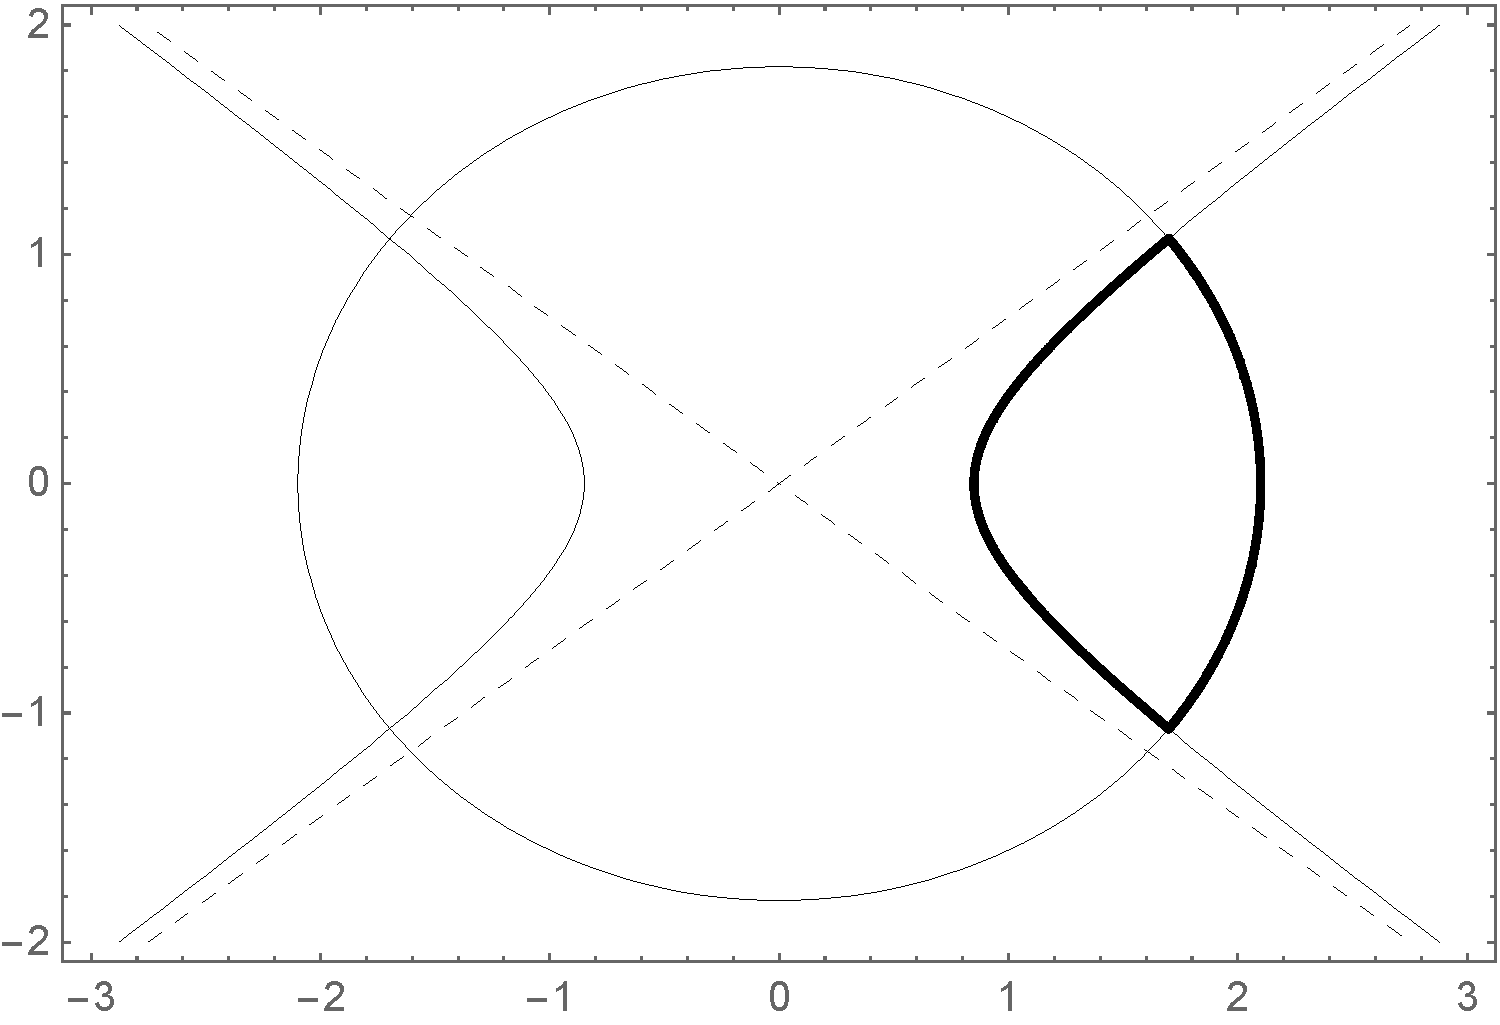
\includegraphics[width=0.8\linewidth]{right1.pdf} \\ 
        Множество $A_\varepsilon$, $\phi_0<\pi/2$
    \end{minipage}
    \hfill
    \begin{minipage}[b][][b]{0.49\linewidth}\centering
        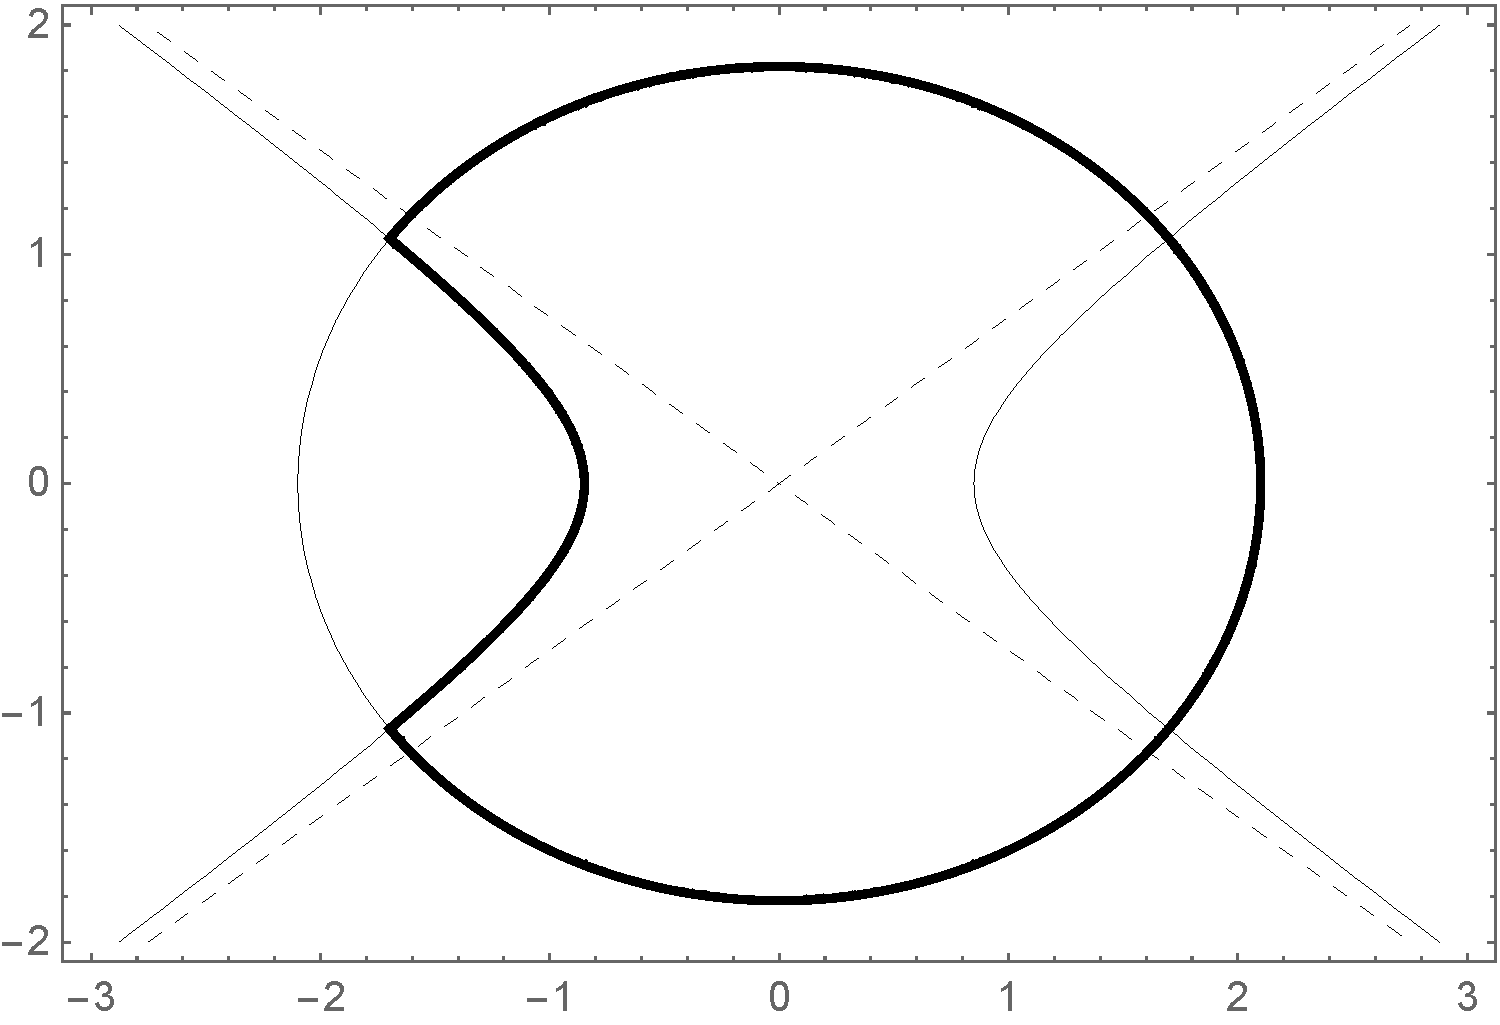
\includegraphics[width=0.8\linewidth]{left1.pdf} \\ 
        Множество $A_\varepsilon$, $\phi_0>\pi/2$
    \end{minipage}
\caption{Примеры множеств $A_\varepsilon$}
\end{figure}

\begin{figure}[ht]
\begin{minipage}{0.9\linewidth}\centering
        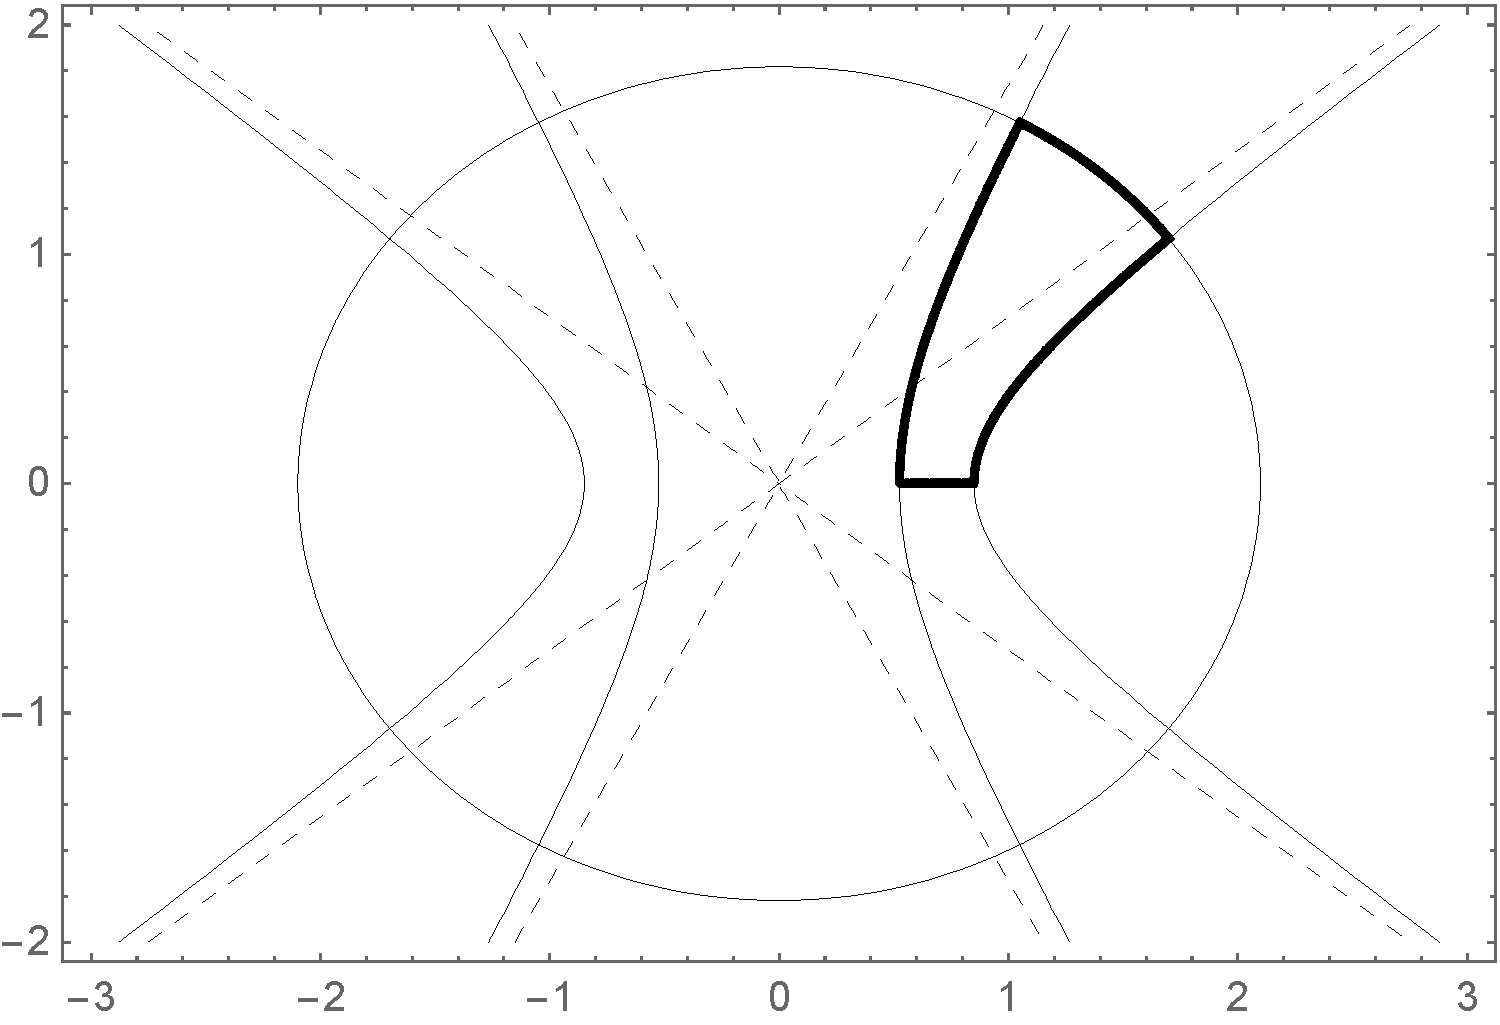
\includegraphics[width=0.8\linewidth]{up1.pdf}  
    \end{minipage}
\caption{        Множество $B_\varepsilon$, $\phi_0<\phi_1<\pi/2$}
\end{figure}

Очевидно, что с приближением величины $\varepsilon$ к 0, эллипс приближается к кругу радиуса $r_0$,
а любая гипербола~(\ref{eq:hyper}) приближается к собственным асимптотам.

Следовательно, при $\varepsilon\to 0$, область $A$ приближается к круговому сектору с величиной центрального угла $2\phi_0$, 
а область  $B$ приближается к круговому сектору с углом $\phi_1-\phi_0$. 


%\subsection{Симметричная область $A_\varepsilon: \rho \in [0,\rho_0], \phi \in [-\phi_0,\phi_0]$}\label{sec:ch2/sec2/sub2}
\subsection{Симметричная область $A_\varepsilon$}\label{sec:ch2/sec2/sub2}
\subsubsection{Собственные функции и асимптотика собственных значений}\label{sec:ch2/sec2/sub2/sub1}

Обозначим через $\Phi_{even}(\zeta, q, \phi), \Phi_{odd}(\zeta, q, \phi)$ четное и нечетное решения уравнения $\frac{\partial^2}{\partial \phi^2}\Phi + (\zeta - 2q\cos{2\phi})\Phi = 0$, соответственно. 
В частности, (см.~\cite{wref2})
\[
\begin{array}{ll}
    \Phi_{even}(a_n(q), q, \phi) = ce_n(\phi, q)	&
    \Phi_{odd}(a_n(q), q, \phi) = fe_n(\phi, q)\\
    \Phi_{even}(b_n(q), q, \phi) = ge_n(\phi, q)	&
    \Phi_{odd}(b_n(q), q, \phi) = se_n(\phi, q)\\
    \Phi_{even}(\lambda_{\nu+2k}(q), q, \phi) = ce_{\nu+2k}(\phi, q) 	&
    \Phi_{odd}(\lambda_{\nu+2k}(q), q, \phi) = se_{\nu+2k}(\phi, q).
\end{array}
\]

Напомним, что эллиптическая система координат имеет особенности на соединяющем фокусы отрезке. Область $A_\varepsilon$ содержит особые точки эллиптической системы координат, а именно, они находятся на отрезке $J$ с концами на правом фокусе и на вершине дуги гиперболы.
Следовательно, решение $\psi(\rho, \phi)$ и его производная должны удовлетворять условиям непрерывности \eqref{eq:disp} и \eqref{eq:grad} на  $J$.
В силу соображений раздела \ref{sec:ch1/sec4/sub2/sub1}, собственная функция  $\psi(\rho,\phi)=R(\rho) \Phi(\phi)$ оператора $\hat{H}$ в области $A_\varepsilon$ является произведением радиальной и угловой функций Матьё одинаковой четности:
$$ \psi(\rho,\phi) = \Phi_{even}(\phi) R_{even}(\rho)  
\text{ или }
 \psi(\rho,\phi) = \Phi_{odd}(\phi) R_{odd}(\rho) .  $$
%\hfill
%$\Box$
То есть, в наших обозначениях в области $A_\varepsilon$ для собственных функций $\psi_{k, m}(\rho, \phi)$ оператора   $\hat{H}$ справедливы выражения
\begin{equation}
\psi_{k, m}(\rho, \phi) = 
\left[
\begin{array}{ll}
    Ce_\nu(\rho, q) ce_\nu(\phi, q) ,   &    \text{нечетный $k \geq 1$}\\
    Se_\nu(\rho, q) se_\nu(\phi, q) ,   &    \text{четный $k \geq 2$}\\
\end{array}
\right.\label{eq:fun}
\end{equation}
с параметрами
\[
\nu = \nu_{k,m} = \nu_0+ \varepsilon^2 \nu_1 + o(\varepsilon^2),  \quad q=q_{k,m} = \dfrac{\varkappa_{k,m}^2 r_0^2 \varepsilon^2}{4},
\]
где
$$\nu_0 = \frac{\pi k}{2\phi_0}\text{\ \  и\  \  }\nu_1=\frac{\alpha_{\nu_0, m}^2}{4} \frac{\pi k \sin 2\phi_0}{\pi^2 k^2 - 4\phi_0^2}  .$$
Для соответствующих собственных  значений  $\varkappa^2_{k, m}$ справедливы равенства
\begin{equation}
\varkappa^2_{k, m} = \dfrac{\alpha_{\nu_0, m}^2}{r_0^2} +
\varepsilon^2 \dfrac{\alpha_{\nu_0, m}^3}{2 r_0^2}\dfrac{\varkappa_1 }{ \left.\frac{\partial J_{\nu_0}(u)}{\partial u}\right|_{u=\alpha_{\nu_0, m}} } + o(\varepsilon^2),\label{eq:val}
\end{equation}
где
\begin{equation*}
    \varkappa_1 = 
    \left[
\begin{array}{ll}
\frac{J_{\nu_0-2}(\alpha_{\nu_0, m})}{4(\nu_0-1)} - \frac{J_{\nu_0+2}(\alpha_{\nu_0, m})}{4(\nu_0+1)} 
  - \nu_1 \left.\frac{\partial J_\nu}{\partial \nu}\right|_{\nu=\nu_0}(\alpha_{\nu_0, m}),\qquad \text{для нечетных $k\geq 3$ ;} \\[10pt]
\frac{(\nu_0 - 2)J_{\nu_0-2}(\alpha_{\nu_0, m})   }{4\nu_0 (\nu_0-1)} -\\
\qquad - \frac{(\nu_0 + 2)J_{\nu_0+2}(\alpha_{\nu_0, m})}{4\nu_0 (\nu_0+1)}  
- \nu_1 \left.\frac{\partial J_\nu}{\partial \nu}\right|_{\nu = \nu_0}(\alpha_{\nu_0, m}), \qquad \ \ \!    \text{для четных $k \geq 2$}.        
\end{array}
\right.
\end{equation*}
Здесь $\alpha_{\nu_0,m}$ --  $m$-й нуль функции Бесселя первого рода $J_{\nu_0}(x)$.


Нечетный и четный случаи мы рассматриваем отдельно. Сперва рассмотрим
\textit{нечетный случай}: $\psi(\rho,\phi) = R_{odd}(\rho)\Phi_{odd}(\phi)  $.

для $\nu \in \mathbb{R} \setminus \{1\}$ 
($\nu=1$ соответствует случаю  $\phi_0=\pi$, который в работе не рассматривается)
справедливо разложение ~\cite[\S 2.2]{wref12},
\begin{align}
\Phi_{odd}(\nu, &{} \phi, q)  = \notag\\
	&{} = \sin{\nu\phi} + 
	\frac{q}{4(\nu-1)} \sin{(\nu-2)\phi} -\frac{q}{4(\nu+1)} \sin{(\nu+2)\phi} + o(q). \label{eq:se}
\end{align}
Напомним, что для $\nu \in \mathbb{R} \setminus \mathbb{Z}$, $\Phi_{odd}(\nu, \phi, q) = se_\nu(\phi, q)$ и для  $\nu \in  \mathbb{Z}$, $\Phi_{odd}(\nu, \phi, q)$ является $se_\nu(\phi, q) $ или $fe_\nu(\phi, q)$ в зависимости от $\nu$, но с тем же разложением (\ref{eq:se}). 
Поэтому, для простоты будем использовать запись $se_\nu(\phi, q)$ вместо $fe_\nu(\phi, q)$, используя только разложения с точностью до $o(q)$. Этот же подход мы будем использовать в дальнейшем без явного упоминания.

Подставим  $\phi=\phi_0$ и $\nu=\nu(q) = \nu_0 + q \nu_1 + o(q)$
в граничное условие $se_{\nu(q)}(\phi_0, q)=0$ угловой функции:
 \begin{align*}
 se_{\nu(q)}(& \phi_0, q) =  \sin \nu_0 \phi_0 + \\
&{} + q \biggl( \nu_1 \phi_0 \cos \nu_0 \phi_0 + \frac{\sin(\nu_0-2)\phi_0}{4(\nu_0-1)}  -\frac{\sin(\nu_0+2)\phi_0}{4(\nu_0+1)} \biggr) + o(q) =0.
\end{align*}
Приравнивая к нулю коэффициенты при каждой степени  $q$, мы получим
\begin{equation*}
\nu_0 = \frac{\pi (2k)}{2\phi_0}, \quad \nu_1 = \frac{\pi (2k) \sin 2 \phi_0}{(\pi^2 (2k)^2 - 4\phi_0^2)}.
\end{equation*}

Рассмотрим второе граничное условие $R(\rho_0) = 0$. 
Для функции  $R(\rho)=Se_\nu(\rho, q)$
справедливо разложение в ряд по функциям Бесселя первого рода, см.~\cite[гл. VIII]{mclachlan}, поэтому:
\begin{multline*}
Se_\nu(\rho, q) \,\propto\,\,  \nu J_\nu(2\sqrt{q} \cosh{\rho})  
+q \bigg( \frac{\nu + 2}{4(\nu+1)} J_{\nu+2}(2\sqrt{q} \cosh{\rho}) - \\
- \frac{\nu - 2}{4(\nu-1)} J_{\nu-2}(2\sqrt{q} \cosh{\rho}) \bigg) + o(q).
\end{multline*}
Символ $\propto$ означает равенство с точностью до умножения на ненулевую константу.

Заметим, что $\frac{1}{\varepsilon} = \cosh \rho = \cosh \rho_0 $, тогда из  $q = \frac{\varkappa^2 r_0^2 \varepsilon^2}{4}$ следует, что $2\sqrt{q} \cosh{\rho_0} =   \varkappa r_0$. 
Для краткости обозначим $u = \varkappa r_0$. Теперь подставим  
$\nu=\nu_0 + q\nu_1 + o(q)$ в граничное условие $0 = Se_{\nu(q)}(\rho_0, q)$:
\begin{multline*}
0 = \nu_0 J_{\nu_0}(u) + q \bigg(  \nu_1 J_{\nu_0}(u) 
- \frac{\nu_0 - 2}{4(\nu_0-1)} J_{\nu_0-2}(u) + %{} \notag\\ 
\\ %&{}+
+ \frac{\nu_0 + 2}{4(\nu_0+1)} J_{\nu_0+2}(u) +
 \nu_0 \nu_1 \left.\frac{\partial J_\nu}{\partial \nu}\right|_{\nu = \nu_0}(u)
\bigg) + o(q).
\end{multline*}
После чего подставим   $u = u_0 + q u_1 + o(q)$ в последнее равенство:
\begin{multline*}
0 = \nu_0 J_{\nu_0}(u_0) + q \bigg( 
\nu_0 u_1 \left.\frac{\partial J_{\nu_0}(u)}{\partial u}\right|_{u=u_0} 
+\nu_1 J_{\nu_0}(u_0) - \frac{\nu_0 - 2}{4(\nu_0-1)} J_{\nu_0-2}(u_0) +\\ 
+\frac{\nu_0 + 2}{4(\nu_0+1)} J_{\nu_0+2}(u_0) 
+ \nu_0 \nu_1 \left.\frac{\partial J_\nu}{\partial \nu}\right|_{\nu = \nu_0}(u_0)
\bigg) + o(q).
\end{multline*}
Снова приравнивая к $0$ коэффициенты при степенях  $q$, получим
\begin{align}
    u_0 =& \alpha_{\nu_0, m}, \label{eq:u0}\\
    u_1 =& \frac{1}{\left.\frac{\partial J_{\nu_0}(u)}{\partial u}\right|_{u=\alpha_{\nu_0, m}} } \biggl(
\frac{(\nu_0 - 2)J_{\nu_0-2}(\alpha_{\nu_0, m}) }{4 \nu_0(\nu_0-1)} - \notag \\    
&{}- \frac{(\nu_0 + 2)J_{\nu_0+2}(\alpha_{\nu_0, m}) }{4 \nu_0(\nu_0+1)} - \nu_1 \left.\frac{\partial J_\nu}{\partial \nu}\right|_{\nu = \nu_0}(\alpha_{\nu_0, m})
    \biggr),\label{eq:u1}
\end{align}
где $\alpha_{\nu_0, m}$ --  $m$-й нуль функции Бесселя $J_{\nu_0}(x)$. 




Из равенства $q=\frac{\varkappa^2 r_0^2 \varepsilon^2}{4}=\frac{u^2 \varepsilon^2}{4}$ можно получить выражение для собственного значения
$$\varkappa_{k, m}^2 = \frac{u^2}{r_0^2} = \frac{u_0^2}{r_0^2} + \frac{2 q u_0 u_1}{r_0^2} + o(q)= \frac{u_0^2}{r_0^2} +  \varepsilon^2 \frac{u_0^3 u_1}{2 r_0^2} + o(\varepsilon^2).$$ 
Из уравнений~(\ref{eq:u0}) и (\ref{eq:u1}) для $u_0, u_1$ верны выражения
\begin{align}
  & \nu_0 = \frac{2\pi k}{2\phi_0},   \nu_1 = \frac{2 \pi k \sin 2 \phi_0}{4 k^2\pi^2  - 4\phi_0^2},\\
   & \varkappa_{k, m}^2 = \frac{\alpha_{\nu_0, m}^2}{r_0^2} 
+  \varepsilon^2 \frac{\alpha_{\nu_0, m}^3}{2 r_0^2}\frac{1}{ \left.\frac{\partial J_{\nu_0}(u)}{\partial u}\right|_{u=\alpha_{\nu_0, m}} } \biggl(
\frac{(\nu_0 - 2)J_{\nu_0-2}(\alpha_{\nu_0, m})   }{4\nu_0 (\nu_0-1)} - \notag \\
&\qquad\qquad{}- \frac{(\nu_0 + 2)J_{\nu_0+2}(\alpha_{\nu_0, m})}{4\nu_0 (\nu_0+1)} - \nu_1 \left.\frac{\partial J_\nu}{\partial \nu}\right|_{\nu = \nu_0}(\alpha_{\nu_0, m})
    \biggr) + o(\varepsilon^2).
 \label{eq:oddSe_nueigenvalues}
 \end{align}


Теперь рассмотрим случай  $\psi(\phi, \rho) = \Phi_{even}(\phi) R_{even}(\rho)$ с \textit{четными} функциями $ \Phi_{even}(\phi) $ и $R_{even}(\rho)$. 
В силу аналогичных соображений, рассмотрим разложение четного решения:
\[
ce_\nu(\phi, q) = 	\cos{\nu\phi} + 
	\frac{q}{4(\nu-1)} \cos{(\nu-2)\phi} -\frac{q}{4(\nu+1)} \cos{(\nu+2)\phi} + o(q).
\]
Используя равенство $ce_\nu(\phi_0, q)=0$ и разложение $\nu = \nu_0 + q \nu_1 + o(q)$,
запишем разложение $ce_\nu$  по степеням $q$:
\begin{multline*}
0=ce_\nu(\phi_0, q) = 	\cos{\nu_0\phi_0}  + \\
+q \biggl(	\frac{\cos{(\nu_0-2)\phi_0}}{4(\nu_0-1)}  -\frac{\cos{(\nu_0+2)\phi_0}}{4(\nu_0+1)} - \nu_1 \phi_0 \sin \nu_0 \phi_0 \biggr) + o(q).
 \end{multline*}
Приравнивая к  $0$ коэффициенты при различных степенях  $q$, получаем
\begin{equation*}
    \nu_0 = \frac{\pi (1 + 2 k)}{2 \phi_0}, \qquad \nu_1 = \frac{\pi (1+2k) \sin 2\phi_0}{\pi^2(1+2k)^2 - 4\phi_0^2}.
\end{equation*}

Чтобы вывести формулу для  $\varkappa^2$, рассмотрим граничное условие $R(\rho_0) = 0$. 
Поскольку $R(\rho) = Ce_\nu(\rho, q)$, можно воспользоваться разложением в сумму по функциям Бесселя первого рода:
\begin{align*}
Ce_\nu(\rho, q) = & J_\nu(2\sqrt{q} \cosh{\rho}) + {}\notag \\
&{}+q \biggl( \frac{1}{4(\nu+1)} J_{\nu+2}(2\sqrt{q}\cosh{\rho}) -\frac{1}{4(\nu-1)} J_{\nu-2}(2\sqrt{q} \cosh{\rho})
\biggr) + o(q).
\end{align*}
Заметим, что $\frac{1}{\varepsilon} = \cosh \rho = \cosh \rho_0 $, тогда из  $q = \frac{\varkappa^2 r_0^2 \varepsilon^2}{4}$ следует, что $2\sqrt{q} \cosh{\rho_0} =   \varkappa r_0$. 
Обозначим для краткости $u = \varkappa r_0$. 

Подставим  $\nu = \nu_0 + q \nu_1 + o(q)$  в граничное условие $0 = Ce_{\nu(q)}(\rho_0, q)$:
\begin{equation}
    0 = 
    J_{\nu_0}(u) + q \biggl( 
    \frac{J_{\nu_0+2}(u)}{4(\nu_0+1)}  - \frac{J_{\nu_0-2}(u)}{4(\nu_0-1)}
    + \nu_1 \left.\frac{\partial J_\nu}{\partial \nu}\right|_{\nu=\nu_0}(u)
    \biggr) + o(q).\label{eq:evenae}
\end{equation}
Теперь подставим $u = u_0 + q u_1 + o(q)$  в полученное выражение~(\ref{eq:evenae}):
\begin{align*}
    &0 =  Ce_{\nu(q)}(\rho_0, q) = 
    J_{\nu_0}(u_0) + q \biggl( 
    u_1 \left.\frac{\partial J_{\nu_0} (u)}{\partial u}\right|_{u=u_0} +  \notag \\
  &\quad{}  + \frac{J_{\nu_0+2}(u_0)}{4(\nu_0+1)} - \frac{J_{\nu_0-2}(u_0)}{4(\nu_0-1)}    + \nu_1 \left.\frac{\partial J_\nu}{\partial \nu}\right|_{\nu=\nu_0}(u_0)
    \biggr) + o(q).
\end{align*}
Из равенства $0$ коэффициентов при каждой степени $q$ следует
\begin{align*}
&u_0 = \alpha_{\nu_0, m}, \\
&u_1 = \frac{1}{\left.\frac{\partial J_{\nu_0} (u)}{\partial u}\right|_{u=\alpha_{\nu_0, m}}} 
\biggl(
\frac{J_{\nu_0-2}(\alpha_{\nu_0, m})}{4(\nu_0-1)} - \frac{J_{\nu_0+2}(\alpha_{\nu_0, m})}{4(\nu_0+1)}
 - \nu_1 \left.\frac{\partial J_\nu}{\partial \nu}\right|_{\nu=\nu_0}(\alpha_{\nu_0, m})
\biggr),
\end{align*}
где $\alpha_{\nu_0, m}$ -- $m$-й нуль функции $J_{\nu_0}(x)$.  

Как и в предыдущем случае, собственное значение
$$\varkappa_{k, m}^2 = \frac{u^2}{r_0^2} = \frac{u_0^2}{r_0^2} + \varepsilon^2 \frac{u_0^3 u_1}{2r_0^2} + o(\varepsilon^2)$$ получается подстановкой значений $u_0, u_1$:
\begin{align*}
&\nu_0 = \frac{\pi (1 + 2 k)}{2 \phi_0}, \quad \nu_1 = \frac{\pi (1+2k) \sin 2\phi_0}{\pi^2(1+2k)^2 - 4\phi_0^2},\\
&\varkappa_{k, m}^2 = \frac{\alpha_{\nu_0, m}^2}{r_0^2} + \varepsilon^2 \frac{\alpha_{\nu_0, m}^3}{2r_0^2} \frac{1}{\left.\frac{\partial J_{\nu_0} (u)}{\partial u}\right|_{u=\alpha_{\nu_0, m}}}\biggl(
\frac{J_{\nu_0-2}(\alpha_{\nu_0, m})}{4(\nu_0-1)} - \notag\\
&\qquad{} - \frac{J_{\nu_0+2}(\alpha_{\nu_0, m})}{4(\nu_0+1)}    - \nu_1 \left.\frac{\partial J_\nu}{\partial \nu}\right|_{\nu=\nu_0}(\alpha_{\nu_0, m})
\biggr) + o(\varepsilon^2).
\end{align*}

\subsubsection{Особый случай: $A_\varepsilon$ для $\phi_0=\pi/2$}\label{sec:ch2/sec2/sub2/sub1}


Для $\nu\ne 1$ формулы для собственных функций и собственных значений, см. уравнения (\ref{eq:fun}) и (\ref{eq:val}), верны. Единственным исключением является случай  $\nu=\nu_0=1$.
Для $\nu=\nu_0=1$ для четного решения справедливо разложение (см. \cite[Subsect.~20.2.27]{wref2}):
\begin{equation*}
ce_1(\phi, q) = 	\cos{\phi}  - \frac{q}{8} \cos{3\phi} + o(q),
 \end{equation*}
для которого граничное условие  $ce_1(\phi_0, q)=0$ выполняется. 
Рассмотрим второе граничное условие $R(\rho_0) = 0$.
Для $R(\rho) = Ce_1(\rho, q)$ существует разложение по функциям Бесселя первого рода:
\begin{equation*}
Ce_1(\rho, q) = J_1(2\sqrt{q} \cosh{\rho}) + \frac{q}{8} J_3(2\sqrt{q}\cosh{\rho}) + o(q).
\end{equation*}
Из подстановок $\cosh\rho = \cosh\rho_0 =  \frac{1}{\varepsilon}$ и $q = \frac{\varkappa^2 r_0^2 \varepsilon^2}{4}$ следует равенство
$2\sqrt{q} \cosh{\rho_0} = 2 \frac{\varkappa r_0 \varepsilon}{2} \frac{1}{\varepsilon} = \varkappa r_0$. Для краткости $\varkappa r_0$ обозначим через $u$. 

Подставим $\nu = 1$ в граничное условие $0 = Ce_1(\rho_0, q)$ и рассмотрим разложение в ряд по степеням   $q$:
\begin{equation*}
    0 = J_1(u) + q \left( \frac{J_3(u)}{8} \right) + o(q).
\end{equation*}
Подстановкой  $u = u_0 + q u_1 + o(q)$ получим:
\begin{equation*}
    0 = 
    J_1(u_0) + q \left( 
    u_1 \left.\frac{\partial J_1 (u)}{\partial u}\right|_{u=u_0}
    + \frac{J_3(u_0)}{8}
    \right) + o(q).
\end{equation*}
Поэтому, 
\begin{equation*}
u_0 = \alpha_{1, m}, \qquad u_1 = 
\frac{ - J_3(\alpha_{1, m}) }{8\left.
\frac{\partial J_1 (u)}{\partial u}\right|_{u=\alpha_{1, m}}},
\end{equation*}
где $\alpha_{1, m}$ -- $m$-й нуль функции Бесселя  $J_1(x)$. По аналогии с предыдущим случаем,
собственное значение $\varkappa_{k, m}^2 = \frac{u^2}{r_0^2} = \frac{u_0^2}{r_0^2} + \varepsilon^2 \frac{u_0^3 u_1}{2r_0^2} + o(\varepsilon^2)$ получается из подстановки величин  $u_0, u_1$:
\begin{align}
   & \varkappa_{k, m}^2 = \frac{\alpha_{1, m}^2}{r_0^2} - \varepsilon^2 \frac{\alpha_{1, m}^3}{16r_0^2} 
    \frac{J_3(\alpha_{1, m})}{\left.\frac{\partial J_1 (u)}{\partial u}\right|_{u=\alpha_{1, m}}} 
    + o(\varepsilon^2), \label{eq:valS1}
    \end{align}



%\subsection{Несимметричная область $B_\varepsilon:  \rho \in [0, \rho_0], \phi \in [\phi_0, \phi_1 ]$}\label{sec:ch2/sec2/sub3}
\subsection{Несимметричная область $B_\varepsilon$}\label{sec:ch2/sec2/sub3}
\subsubsection{Собственные функции и асимптотика собственных значений}\label{sec:ch2/sec2/sub3/sub1}


Внутренность области $B_\varepsilon$ не содержит особых точек эллиптической системы координат~(\ref{eq:coord}). Поэтому, условия непрерывности сдвига или непрерывности производной, рассмотренные для случая симметричной области (в частности, для эллипса), здесь не требуются.
Хотя эти особые точки, тем не менее, появятся на границе  $B_\varepsilon$ (а именно, они образуют горизонтальный отрезок в составе границы).

Рассмотрим собственную функцию $\psi_{k,l}(\rho,\phi) = R(\rho)\Phi(\phi)$.
Обращение  $\psi_{k,l}(\rho,\phi) $ в нуль на горизонтальном отрезке на границе  $B_\varepsilon$
подразумевает, что $\psi_{k,l}(\rho,\phi)$ может быть представлена в виде
\[
\psi(\rho,\phi) = 
    \left(
    \Phi_{even}(\phi_0) \Phi_{odd}(\phi) - \Phi_{even}(\phi) \Phi_{odd}(\phi_0) 
    \right) R_{odd}(\rho).
\]

%{\em Далее следует основной результат текущего подраздела.}
В области  $B_\varepsilon$ для собственных функций $\psi_{k, m}(\rho, \phi)$ и собственных значений $\varkappa^2_{k, m}$ оператора $\hat{H}$ справедливы выражения

\begin{align}
&\psi_{k, m}(\rho, \phi) = 
    Se_\nu(\rho, q) \biggl( ce_\nu(\phi_0, q) se_\nu(\phi, q) -ce_\nu(\phi, q) se_\nu(\phi_0, q) \biggr) ,  \label{eq:funB}
\end{align}
с параметрами
\begin{align*}    
    & q=q_{k,m} = \frac{\varkappa_{k,m}^2 r_0^2 \varepsilon^2}{4}, \\ 
&\nu = \nu_{k,m} = \frac{\pi k}{\phi_1-\phi_0} +\varepsilon^2 \frac{\alpha_{\nu_0, m}^2}{4} \frac{\pi k (\sin 2\phi_1 - \sin 2 \phi_0)}{\pi^2k^2-(\phi_1-\phi_0)^2} + o(\varepsilon^2) ,  
\end{align*}
где
\begin{align*}
& \nu_0 = \frac{\pi k}{\phi_1-\phi_0},\text{\ \ и \ \ }
\nu_1= \frac{\pi k (\sin 2\phi_1 - \sin 2 \phi_0)}{\pi^2k^2-(\phi_1-\phi_0)^2} .
\end{align*}
Для соответствующих собственных значений справедливы равенства
\begin{align}
\varkappa_{k, m}^2 ={}& \frac{\alpha_{\nu_0, m}^2}{r_0^2} +  \varepsilon^2 \frac{\alpha_{\nu_0, m}^3}{2 r_0^2}\frac{1}{ \left.\frac{\partial J_{\nu_0}(u)}{\partial u}\right|_{u=\alpha_{\nu_0, m}} }  
 \biggl(\frac{(\nu_0 - 2)J_{\nu_0-2}(\alpha_{\nu_0, m})   }{4\nu_0 (\nu_0-1)} -
\notag \\ 
&{}- \frac{(\nu_0 + 2)J_{\nu_0+2}(\alpha_{\nu_0, m})}{4\nu_0 (\nu_0+1)} 
- \nu_1 \left.\frac{\partial J_\nu}{\partial \nu}\right|_{\nu = \nu_0}(\alpha_{\nu_0, m})
    \biggr) + o(\varepsilon^2).\label{eq:valB}
\end{align}
Здесь $\alpha_{\nu_0,m}$ -- $m$-й нуль функции Бесселя первого рода $J_{\nu_0}(x)$.


Мы хотим найти решение углового решения в виде
\begin{multline*}
\Phi(\phi, q) = \Phi_{even}(\phi_0) \Phi_{odd}(\phi) - \Phi_{even}(\phi) \Phi_{odd}(\phi_0)  = \\
=ce_\nu(\phi_0, q) se_\nu(\phi, q) - ce_\nu(\phi, q) se_\nu(\phi_0, q).
\end{multline*}

 
Подстановим $\nu(q) = \nu_0 + q \nu_1 + o(q)$
в граничное условие  $\Phi(\phi_1, q) = 0$
и из разложения функций $ce_\nu(\phi, q)$ и $se_\nu(\phi, q)$, в ряды по степеням  $q$
 получим
\begin{multline*}
0=\Phi(\phi_1, q) = ce_\nu(\phi_0, q) se_\nu(\phi_1, q) -ce_\nu(\phi_1, q) se_\nu(\phi_0, q) = \\
= \sin \nu_0 (\phi_1 - \phi_0) +q \biggl(
\frac{1}{4(\nu_0+1)}  \sin{(2 \phi_0 + \nu_0(\phi_0-\phi_1))}+  \\
+\frac{1}{4(\nu_0+1)} \sin{(\nu_0(\phi_0-\phi_1)-2\phi_1)} - \\
-\frac{1}{2(\nu_0-1)}\cos{(\phi_0 + \phi_1)}\sin{(\nu-1)(\phi_0-\phi_1)} -\\
- \nu_1 (\phi_0 - \phi_1) \cos{\nu_0(\phi_0-\phi_1)} \biggr) + o(q).
\end{multline*}
Следовательно, 
\begin{equation*}
    \nu_0 = \frac{\pi k}{\phi_1-\phi_0}, \qquad \nu_1 = \frac{\pi k (\sin 2\phi_1 - \sin 2 \phi_0)}{\pi^2k^2-(\phi_1-\phi_0)^2}.
\end{equation*}

Из соображений, аналогичных тем, что были проведены для  $\psi_{k, m}(\rho, \phi) = \Phi_{odd}(\phi) R_{odd}(\rho)$ из предыдущего подраздела,
мы получаем разложение радиальной функции и соответствующих собственных значений:
\begin{align*}
    \varkappa_{k, m}^2 ={}& \frac{\alpha_{\nu_0, m}^2}{r_0^2} +  \varepsilon^2 \frac{\alpha_{\nu_0, m}^3}{2 r_0^2}\frac{1}{ \left.\frac{\partial J_{\nu_0}(u)}{\partial u}\right|_{u=\alpha_{\nu_0, m}} }\biggl(\frac{(\nu_0 - 2)J_{\nu_0-2}(\alpha_{\nu_0, m})   }{4\nu_0 (\nu_0-1)} - \notag \\
&{}- \frac{(\nu_0 + 2)J_{\nu_0+2}(\alpha_{\nu_0, m})}{4\nu_0 (\nu_0+1)}  - \nu_1 \left.\frac{\partial J_\nu}{\partial \nu}\right|_{\nu = \nu_0}(\alpha_{\nu_0, m})
    \biggr) + o(\varepsilon^2).
\end{align*}

\subsubsection{Особые случаи: $B_\varepsilon$ для $(\phi_0, \phi_1)=(0,\pi)$ и для $(\phi_0, \phi_1)=(0,\pi/2)$}\label{sec:ch2/sec2/sub3/sub2}


Хотя $\phi_0=0, \phi_1=\pi/2$ является особенным случаем при $k=1$,
несложно проверить, что уравнения (\ref{eq:funB}) и (\ref{eq:valB}) выполняются.

Для  $\phi_0=0, \phi_1=\pi$
особенным является случай  $k=1$ (следовательно, $\nu_0=1$). 
Для остальных величин $k$ равенства (\ref{eq:funB}) и (\ref{eq:valB}) справедливы.
Теперь предположим $k=1$ (и $\nu=\nu_0 = 1$).
Тогда для соответствующего нечетного решения углового уравнения справедливо разложение  (см. \cite[Subsect.~20.2.27]{wref2})
\begin{equation*}
se_1(\phi, q) = 	\sin{\phi}  - 	\frac{q}{8} \sin{3\phi} + o(q),
 \end{equation*}
для которого выполняется граничное условие $se_1(\phi_0, q)=0$. 
Теперь рассмотрим второе граничное условие $R(\rho_0) = 0$. 
Для функции $R(\rho) = Se_1(\rho, q)$ справедливо разложение по функциям Бесселя первого рода:
\begin{equation*}
Se_1(\rho, q) = J_1(2\sqrt{q} \cosh{\rho}) + \frac{3 q}{8} J_3(2\sqrt{q}\cosh{\rho}) + o(q).
\end{equation*}
Подставим $\cosh \rho = \cosh \rho_0 =\frac{1}{\varepsilon}$.
Тогда из $q = \frac{\varkappa^2 r_0^2 \varepsilon^2}{4}$ следует равенство
$2\sqrt{q} \cosh{\rho_0} =  \varkappa r_0$.

Для краткости положим $u = \varkappa r_0$ .
Подставим $\nu = 1$ в граничное условие радиальной функции и разложим ее в ряд степенной ряд по $q$:
\begin{equation*}
    0 = Se_1(\rho_0, q) = 
    J_1(u) + q  \frac{3 J_3(u)}{8} + o(q).
\end{equation*}
Теперь подставим $u = u_0 + q u_1 + o(q)$:
\begin{align*}
    0 = Se_1(\rho_0, q) =    J_1(u_0) + q \left( 
    u_1 \left.\frac{\partial J_1 (u)}{\partial u}\right|_{u=u_0}
    + \frac{3 J_3(u_0)}{8}
    \right) + o(q).
\end{align*}
Отсюда 
\begin{equation*}
u_0 = \alpha_{1, m}, \qquad u_1 = 
\frac{ - 3 J_3(\alpha_{1, m}) }{8\left.
\frac{\partial J_1 (u)}{\partial u}\right|_{u=\alpha_{1, m}}},
\end{equation*}
где $\alpha_{1, m}$ -- $m$-й нуль функции $J_1(x)$. 

Наконец, как в предыдущем случае, подстановкой $u_0, u_1$ в $\varkappa_{1, m}^2 = \frac{u^2}{r_0^2} = \frac{u_0^2}{r_0^2} + \varepsilon^2 \frac{u_0^3 u_1}{2r_0^2} + o(\varepsilon^2)$, получим выражение для собственного значения:
\begin{align}
    \varkappa_{1, m}^2& = \frac{\alpha_{1, m}^2}{r_0^2} - \varepsilon^2 \frac{3\alpha_{1, m}^3}{16r_0^2} 
    \frac{J_3(\alpha_{1, m})}{\left.\frac{\partial J_1 (u)}{\partial u}\right|_{u=\alpha_{1, m}}} 
    + o(\varepsilon^2).  \label{eq:valS2}
\end{align}



\FloatBarrier
